\documentclass[12pt,a4paper]{article}
\RequirePackage[french]{babel}
\usepackage{fancyhdr}
\usepackage[latin1]{inputenc}
\usepackage{amsfonts}
\usepackage[french]{babel}
\usepackage{listings}
\usepackage{setspace}
\usepackage{graphicx}
\usepackage[T1]{fontenc}
\usepackage{geometry}
\geometry{vmargin=3.5cm,hmargin=2.25cm}
\pagestyle{plain}

\selectlanguage{french}

\begin{document}
\chead{Aegina : rapport de soutenance \no 1}
\begin{titlepage}
\begin{center} 
\huge
\vspace*{5cm}
Aegina : rapport de soutenance \no 1\\
\vspace*{2em}
\large
Florian \bsc{Amsallem} (amsall\_f) , Th�o \bsc{Issarni} (issarn\_t), \\Julien \bsc{Mounier} (mounie\_a), Romain \bsc{Mounier} (mounie\_r)\\
\vspace{2em}
AIM$^{2}$\\
\vspace{2cm}
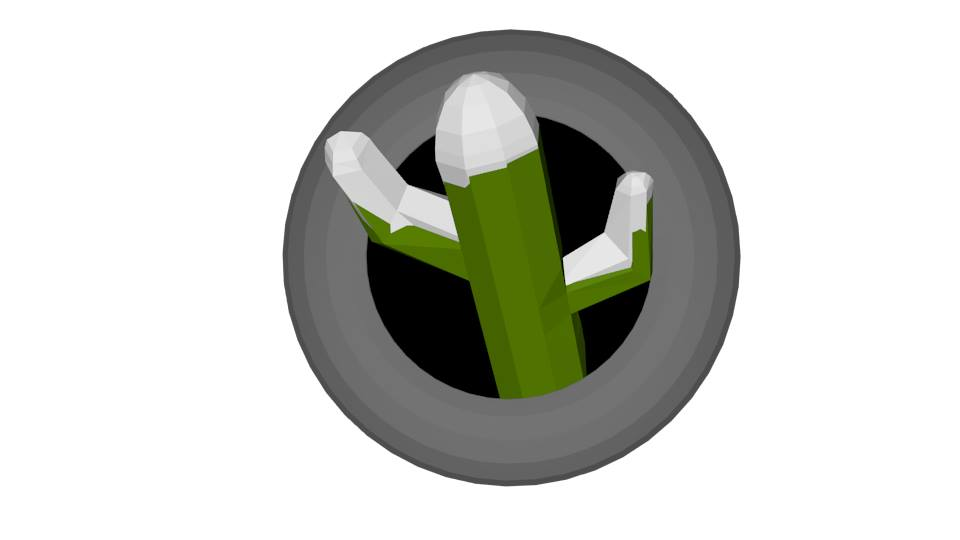
\includegraphics[width=12cm]{logo.jpg}
\end{center} 
\end{titlepage}
\onehalfspacing
\tableofcontents
\pagebreak

\section*{Introduction}
\pagebreak
\addcontentsline{toc}{section}{\protect\numberline{}Introduction}

\section{Concepts et r�flexions}

\subsection{Gameplay}

\subsection{Univers du jeu}

\subsubsection{Aegina}

\subsubsection{Il}

\subsubsection{Le floatium et le sunkium}


\pagebreak

\section{r�alisation}

\subsection{Pr�-janvier}

\subsubsection{Cycle jour/nuit (Julien)}

\subsubsection{Inventaire (Romain et Florian)}

\subsubsection{Animation 3D (Th�o)}

\subsubsection{D�placement du personnage et de sa camera (Th�o et Julien)}

\subsubsection{models 3D (Julien)}


\subsection{Janvier}

\subsubsection{barre de selection (Florian)}

\subsubsection{menus (Romain et Florian)}

\subsubsection{Class \textit{Item} (Romain)}

\subsubsection{Multi-joueurs (Florian)}

\subsubsection{Son (Th�o et Romain)}


\subsection{F�vrier}

\subsubsection{G�n�ration al�atoire (Florian et Julien)}

\subsubsection{Drop d'Item (Florain et Julien)}

\subsubsection{Biblioth�que (Florian, Romain et Th�o)}

\subsubsection{Histoire (Romain et Th�o)}


\subsection{Mars}

\subsubsection{Int�raction avec l'environnement (Florian et Julien)}

\subsubsection{Cristal (Romain et Julien)}

\subsubsection{Chat (Florian)}

\subsubsection{Musique (Th�o)}

\subsubsection{Survie (Th�o)}

\subsubsection{Alpha (Florian)}

\pagebreak

\section{pr�vision}

\subsection{Les quatre grand axe}

\subsubsection{Creation d'objet}

\subsubsection{Ajout des cr�atures}

\subsubsection{Ajout des succ�s}

\subsubsection{PVP et Conqu�te}


\subsection{Les am�liorations}

\subsubsection{Survie}

\subsubsection{G�n�ration al�atoire}

\subsubsection{Histoire}

\subsubsection{Environnement sonore}

\subsubsection{Personnage}

\pagebreak

\section*{Conclusion}
\addcontentsline{toc}{section}{\protect\numberline{}Conclusion}
\end{document}
